\documentclass[conference]{IEEEtran}

\ifCLASSINFOpdf

\else

\fi


\usepackage{graphicx}
\usepackage{textcomp}

% correct bad hyphenation here
\hyphenation{op-tical net-works semi-conduc-tor}


\begin{document}
 
\title{Competitive co-evolution in robots: \\ heterogeneity vs homogeneity}



\author{\IEEEauthorblockN{Enrico Rotundo, Selene Beaz Santamaria, Andrea Jemmet, Tommie Kerstens}
\IEEEauthorblockA{
Vrije Universiteit Amsterdam \\
Amsterdam, Netherlands}}



\maketitle


\begin{abstract}
In the context of robotics, intelligent behaviours are often achieved using neural networks as controllers evolved using  an evolutionary algorithm.
In the case of multiple individuals within a species, controllers can be either homogeneous or heterogeneous.
In this paper, we use competitive co-evolution of homogeneous and heterogeneous controllers in order to investigate its effects on the emergence of specialisation behaviour regarding a herding task.
% TODO: add what we have discovered
\end{abstract}


\IEEEpeerreviewmaketitle


\section{Introduction}
Evolutionary algorithms (EA) are biology inspired algorithms that, going through multiple steps (e.g., generation, procreation, etc.), are able to evolve entities over time.
Thus, the entities subject to the evolution are referred to as individuals,
%and the EA acts as the digital environment these individuals are born, live, procreate and die in.
and the evolution is usually controlled such that next generations improve along the runs.
In the field of robotics, EAs can be used to evolve the behavioural controller of a robot, these controllers are evolved as individuals in an EA.
A Neural Network (NN) is a function estimator that can be used as a controller and its design is natural inspired by the biological nervous system.
In order to employ a NN as a controller, inputs usually come from the sensors making observations of the environment, while the weights are evolved by an EA.
The complete evolutionary process can be run in a simulation which exploits the computer's computational power in order to evaluate many individuals in a reasonable time. 
Robotics employs both EAs and NNs in order to evolve intelligent behaviours that can pursue one or more given goals.

Tasks composition and complexity can vary based on the specific scenario, in general it is subject of many studies aiming to solve different tasks.
For instance, tasks can be relatively small (e.g., moving objects) or more based on collaboration between a number of individuals.
Research investigates collective behaviour in order to asses to which extent collaboration between individuals is feasible.  

In this paper, we consider competitive co-evolution within a herding task which consists of a number of shepherds that herd a sheep into a corral.
We evolve NN controllers and assign them to the agents, the latter step can be done with the homogeneous or heterogeneous approach.
While the former employs the same controller instance for each agent, 
%meaning that each shepherd is assigned to the same controller. 
%This one single controller is also the only evolved individual in the EA. 
in the latter each agent gets its own instance of a controller, which is separately evolved by an EA.
% TODO are we going to talk about increasing complexity here?
Moreover, the task complexity can be increased by varying or introducing new agents like adding a fox.

In this paper we employ the aforementioned components within a simulated herding task.
Thus, we recap our objectives in the following list:

\begin{itemize}
	\item To compare homogeneity versus heterogeneity.
	\item To estimate the effect on homo versus heterogeneity of increasingly difficult task.
 	\item To develop controlled experiments through software simulations, using ad hoc libraries.
	\item To collect comprehensive results data.
\end{itemize}
 
\subsection{Research questions}
In the herding task, shepherds and sheep have opposing goals.
While the former tries to herd sheep into the corral, the latter tries to escape through the left side of the pasture. 
Thus, species can be competitively co-evolved in a race to evolve strategies to accomplish opposing goals. 
Furthermore, the task complexity can be influenced by varying different parameters such as the number of present agents per each type or their relative movement speeds. 
Another type of dimension used to scale the difficulty is the type of controller used,
Instances of different controller types can be either \textit{static} or \textit{intelligent}.
A \textit{static} controller is simply a predefined set of rules that implements a specific behaviour.
Although an \textit{intelligent} controller is more complex, it is able to  adapt itself over time.
In this paper both the sheep and the shepherds have an \textit{intelligent} controller.
The intelligence of the controller is based on the assumption that since a NN is evolved, the controller has the possibility to adapt to its environment through the evolutionary process. 
This process, in which many strategies are simulated and evaluated, is comparable to a learning process and enables adaptivity. 
Assuming an intelligent sheep we state the following research questions:
 
\begin{enumerate}
	\item How does the competitive co-evolution affect the relation between homogeneous and heterogeneous shepherds' controllers, in a co-evolved herding task?
	\item How does increasing the difficulty (e.g.: by incrementing the sheep’s speed) of a single task increases the necessity for heterogeneous controllers?
	\item How does increasing task complexity by adding more sheep affects the effectiveness of herding?
\end{enumerate}

\subsection{Hypothesis}
\label{sec:hypothesis}
The following hypothesis are in one to one relationship with the aforementioned research questions:

\begin{enumerate}
	\item Shepherds' fitness in the heterogeneous case is overall higher than in the homogeneous case.
	\item Shepherds' fitness in the heterogeneous case and sheep’s speed are inversely related, such that fitness decreases as speed increases.
	\item Shepherds' fitness in the heterogeneous case and sheep’s multiplicity are inversely related, such that fitness decreases as speed increases.
\end{enumerate}

We now consider $H_1$ and we leave the testing of the others as future work. 
The $H_0$, namely null hypothesis, is ``Shepherds’ fitness in the heterogeneous case is equivalent to the one of the homogeneous''.

\section{Literature}
 
\subsection{Co-evolution}
The effects of co-evoultion in butterflies and plants have been studied as early as 1964 in ~\cite{ehrlich1964butterflies}.
Furthermore, the authors of ~\cite{janzen1980coevolution} define co-evolution as ``an evolutionary change in a trait of the individuals in one population in response to a trait of the individuals of a second population''.
%In 1980 Janzen's \cite{janzen1980coevolution} formalised a clear definition for coevolution:
%`` 'Coevolution' may be usefully defined as an evolutionary change in a trait of the individuals in one population in response to a trait of the individuals of a second population, followed by an evolutionary response by the second populations to the change in the first.''


\subsection{Competitive Co-evolution}
Dawkins and Krebs describe in~\cite{dawkins1979arms} the dynamics and the terminology for competitive coevolution by providing examples of manifestations of competitive coevolution in natural systems.
In~\cite{stanley2004competitive}, the authors show that through the complexification of agent controllers in a competitive co-evolutionary setting, the controller's added complexity can be utilized through the generation of more advanced strategies as complexity increases.


\subsection{Homogeneity vs Heterogeneity in ANN's}
\cite{potter2001heterogeneity} performed a study to a tradeoff of homogeneity versus heterogeneity in the control systems of robots by allowing teams to coevolve their high-level controllers given different levels of difficulty of the task
Hypothesised was that: ``\textit{simply increasing the difficulty of a task is not enough to induce a team of robots to create specialists.}''
Task difficulty was varied by replacing one adversary's passive controller with an active variant supposedly proving that increased difficulty did not justify the use of heterogeneous controllers.
However, increased difficulty was never implemented structurally nor tested methodologically. 



\section{Model}
Our model is based on Potter et al. work \cite{potter2001heterogeneity}. The task domain relates to a herding task that simulates shepherd robots trying to push sheep robots into a corral. The environment consists of a 37 x 37 foot pasture with fences on the top and bottom; the corral is positioned on the right side, and the pasture is open on the left side for the sheep to escape.

We module the task complexity by controlling the number of agents of each type that take part in the task. Thus, we operationalize it as the sheep to dog ratio, with increased ratio implying a more complex task for the shepherds.
 
We compute the center of sheep - which is equal to the position of the sheep when there is only one - and take is as center for a polar coordinate system. Therefore, the first component for a coordinate is the distance to the center, called the range. The axis is created between this center and the midpoint for the entrance of the corral, from which angles are created for the second component of the polar coordinates, called bearings. 



\subsection{NN design}
The controllers for the agents are composed of feed forward neural networks, with each agent containing a multiplayer perceptron with one hidden layer. The inputs for the networks come in pairs as the range and bearing of other agents in the polar coordinate system previously described. In a simple network, where an agent can only see one other agent, the network consists of two input nodes and a bias, and its hidden layer has three nodes. Alternatively, if the agent can see two other agents it has a more complex neural network, with four input nodes and a bias, and five nodes in its hidden layer. 

The activation function a sigmoid function centered at 0. The output of the network represents the coordinates where the agent will try to move to in the next time step. Since the output has a range from (0, 1), it must be translated into a range of [0, 37] for the ratio and [-pi, pi] for the bearing. 
 

\subsection{Evolution of NN controllers}
The algorithm used to evolve the controllers follows the frameworks of evolutionary strategies. The genome is an array of doubles consisting of the weights for the neural network: 17 for a simple network and 37 for a complex network. The specific strategy is mu + lambda, with mu = 10 and lambda = 100. The survivor selection mechanism is tournament selection with size 5. 

In order to calculate the fitness for an individual, all controllers are evaluated through 10 trials of the task and the average is taken as fitness. Every trial runs for a maximum of 2.5 simulated time steps, unless all but one sheep escape or get corralled, in which case the simulation stops. In cases where there is only one sheep, the sheep must be corralled or has to escape in order for the simulation to stop before the time expires.

Different fitness functions are determined for each type of agent. On the one hand, the fitness for the shepherds is determined as the total distance from every sheep to the corral, added during the simulation time steps. Individual bonuses are giving to specific shepherd agents for bumping sheep and group penalties are assigned to all shepherds for letting sheep escape. The range for this function is [-X, 0]. 

On the other hand, the fitness for a sheep is determined as its own distance to the corral over the simulation time steps. In scenarios where there are more than one sheep, a group component is added to motivate sheep to stay in groups. This is composed as the ratio of the group added over the simulation time steps. This ratio is calculated as the ration from the furthest sheep to the center of the sheep in a specific time step. The range for this function is [0, +X]

Both functions are set up as maximization problems. 

In homogeneous set ups, we evolve one controller per type of agent, meaning we have two subpopulations, one for shepherds and one for sheep, coevolving. However, to create heterogeneity a population per agent is created. For example, in a scenario with two shepherds and one sheep, there is a total of three subpopulations, two of them cooperating among each other and competing with the third one.  



\subsection{Shepherds controllers}
The inputs for the shepherd controllers are the information about the closest shepherd and the closest sheep. Thus, its inputs are 

\begin{enumerate}
	\item closestSheep\_r
	\item closestSheep\_b
	\item closestShepherd\_r
	\item closestShepherd\_b 
\end{enumerate}

The third and fourth input are not taken into account in scenarios where there is only one shepherd. 

We assume the shepherds need to evolve cooperation behaviours among themselves to successfully herd the sheep, but competitive behaviours against sheep who want to escape. To achieve the first objective, a shepherd needs information about the other shepherds around. However, in an attempt to be realistic and keep the network complexity low, we only provide the controller with information for the closest shepherd. Similarly, to achieve the second objective a shepherd needs information about the sheep. Following the same motivation, only the closest sheep position is fed into the network. 
. 

\subsection{Sheep controllers}
The sheep controllers are determined in a similar way. Once again, the inputs take information about the closest sheep and closest shepherd. Thus, we have the inputs as 
\begin{enumerate}
	\item closestShepherd\_r
	\item closestShepherd\_b
	\item closestSheep\_r
	\item closestSheep\_b
\end{enumerate}



Once again, the third and fourth inputs are not taken into account in scenarios where there is only one sheep. 

The assumption for competitive and cooperative collective behaviour still holds. This time, in order to avoid the shepherd and be able to escape, sheep must have information about the closest shepherd. Yet, they also have a strong preference to stay in a group and so need information about the closest sheep around them in order to pursue this goal. 

%talk about homo or hetero controllers


\section{Implementation}
The project is coded in Java with use of Mason for handling agents and their movements, In order to introduce evolutionary computing, we combine it with ECJ. We use neuroph as the library for neural networks. 

\subsection{Obstacle avoidance}
Given the output of the networks, the agents will try to move into a position, however, both types of agents have obstacle avoidance built into their behaviour which might prevent them from moving to the target position. Shepherds avoid bumping into fences, the corral or other agents within a 3 simulation unit ratio. Meanwhile, the sheep can only avoid fences and other agents within a 2 simulation unit ratio. 

\subsection{Interpreting the NN output}
Since the output for the network is represented as polar coordinates centered at the sheep center of mass, they have to be translated into Cartesian coordinates in the pasture. 


\section{Experiment}
\label{sec:experiment}
In this section we detail the design of the experiments performed in this paper. In order to test our hypothesis, we perform coevolution across 100 generations. We run the simulation 40 times and perform statistical analysis to get 95\% confidence intervals.


We first consider the experiments that relate to $H_1$ listed in ~\ref{sec:hypothesis}. To investigate the difference between homogeneous and heterogeneous controllers for the shepherd agents, we first explore a scenario with two shepherd and one sheep. 
\begin{itemize}
	\item 2 homogeneous shepherd’s vs 1 (intelligent) sheep
	\item 2 heterogeneous shepherd’s vs 1 (intelligent) sheep
\end{itemize}
 
 Later on, we compare different scenarios with different number of dogs corralling one sheep. This way the task complexity varies by having different sheep to dog ratios. 


\section{Results}
In this section we present the results of the experiment detailed in Section ~\ref{sec:experiment}.

\begin{figure}[ht]
\centering
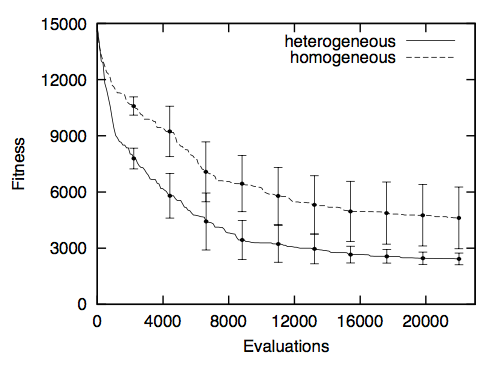
\includegraphics[width=3.3in]{imgs/homo_vs_hetero.png}
\caption{TODO.}
\label{fig:homo_vs_hetero}
\end{figure}

\section{Conclusion}
The conclusion goes here.

\subsection{Future work}
TODO

-In a competitive co-evolution, how does increasing task complexity by adding more sheep affects the effectiveness of herding? %TODO: fix

-[In a competitive co-evolution, do heterogeneous sheep perform better than homogeneous?] %TODO: fix



\bibliographystyle{abbrv}
\bibliography{bibliography}



\end{document}

